\documentclass[10pt]{article}
\usepackage[utf8]{inputenc}
\usepackage[T1]{fontenc}
\usepackage{graphicx}
\usepackage[export]{adjustbox}
\graphicspath{ {./images/} }
\usepackage{amsmath}
\usepackage{amsfonts}
\usepackage{amssymb}
\usepackage[version=4]{mhchem}
\usepackage{stmaryrd}
\usepackage{multirow}

\begin{document}


\section{Contexte}
Dans la volonté de rééducation à la marche des patients partiellement ou totalement paralysés au niveau des membres inférieurs, les exosquelettes de marche offrent une solution de plus en plus envisagée par les structures de soins. Si les technologies existantes permettent des séances de rééducation musculaire efficaces, elles n'offrent pour le moment que peu de possibilités d'amélioration dans la vie quotidienne des patients, du fait de la nécessité de la présence d'un personnel soignant formé à leur utilisation.

Il apparait ainsi qu'une solution permettant une plus grande autonomie des patients, que ce soit pour des séances de rééducation encadrées, ou pour leurs déplacements dans la vie quotidienne serait une grande avancée. Elle permettrait ainsi des fréquences, intensités et durées de séances plus en phase avec la pathologie de la personne équipée, tout en facilitant sa mobilité au quotidien.

Pensé pour minimiser le temps de formation pour le patient et le thérapeute, l'exosquelette Atalante (figure 1), développé par la société Wandercraft a pour volonté d'optimiser les séances de rééducation, et à terme d'aboutir à une solution permettant l'autonomie quasi totale du patient. En effet, ce système permet la verticalisation et des déplacements pouvant s'affranchir de toute dépendance à une tierce personne. De par sa liberté d'utilisation pour le patient, les bénéfices sont importants : possibilité de retours sensoriels, flexibilité de l'entrainement à la marche et à la course ou encore personnalisation des programmes proposés.
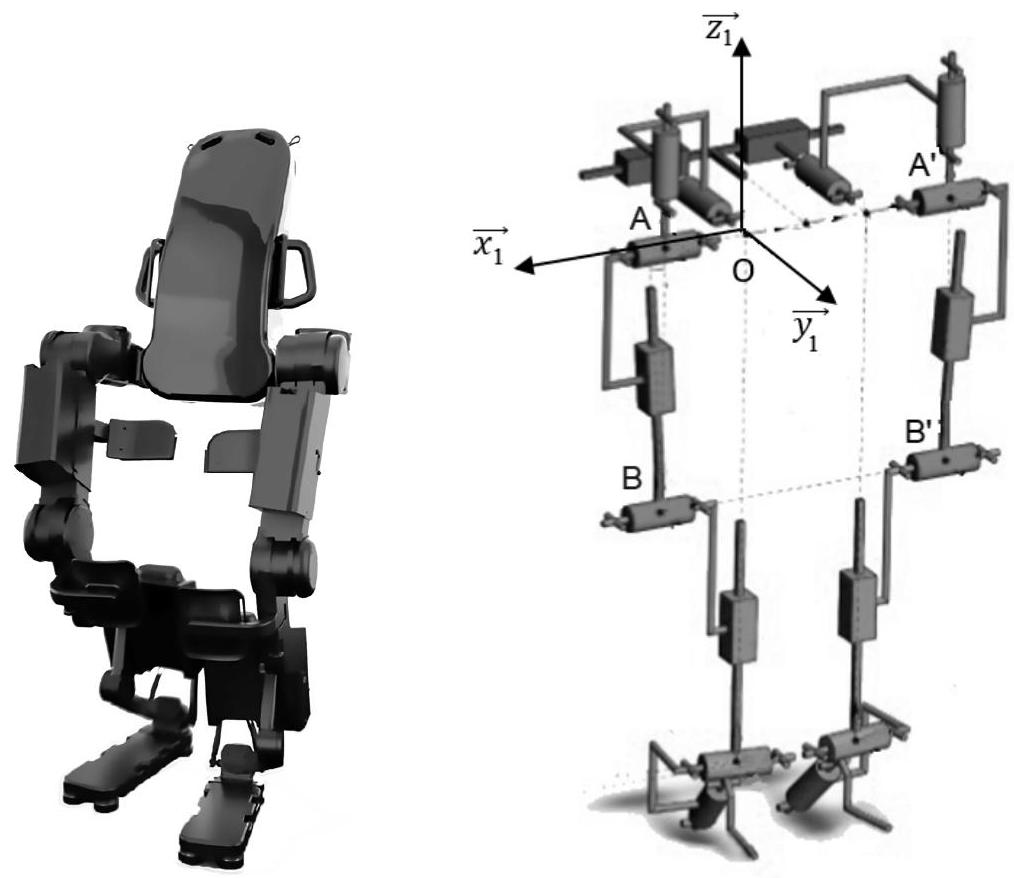
\includegraphics[max width=\textwidth, center]{2023_05_12_54c6a64d2ffce28d5c72g-01(1)}

Figure 1 Exosquelette Atalante et modélisation 3D associée

L'architecture de l'exosquelette autorise la complète autonomie des membres supérieurs du patient. De plus, le réglage rapide des dimensions des jambes et des tibias de l'exosquelette et une utilisation intuitive de son paramétrage permettent une utilisation plus aisée. Ainsi, associé avec la possibilité de variation de l'aide apportée par les différents actionneurs, cet équipement est en parfaite adéquation avec l'enchainement des séances de rééducation où les déplacements sont totalement pris en charge, quelles que soient la pathologie et la morphologie du patient.

Les exercices programmés par les thérapeutes s'articulent autour de deux stratégies thérapeutiques différentes, selon le handicap du patient :

\begin{itemize}
  \item la proprioception (sa propre perception) de la verticalité et de la marche pour les patients paraplégiques ou ayant des problèmes d'équilibre ;

  \item le renforcement musculaire pour les patients ayant subi un traumatisme important. Afin de permettre au patient de reproduire une marche comparable à celle d'un humain valide, et ce quel que soit l'exercice de rééducation préprogrammé, l'exosquelette Atalante possède douze degrés de liberté, six par jambe, et chaque mobilité est contrôlée par un actionneur électrique.

\end{itemize}

L'ensemble de l'étude menée dans ce sujet se limitera à une marche en ligne droite (figure 3), dans le plan sagittal tel que défini figure 2.

La loi de commande des actionneurs associés aux différentes articulations est donc conditionnée par :

\begin{itemize}
  \item les trajectoires des différents membres lors de la marche, prédéterminées par un serveur extérieur lors de la prise de mesures du patient ;

  \item la stabilisation du patient lors de la marche;

  \item la rééducation musculaire du patient, selon un protocole dicté par le thérapeute.

\end{itemize}

Le cahier des charges partiel de l'exosquelette à vérifier dans ce sujet est fourni en annexe A.

\begin{center}
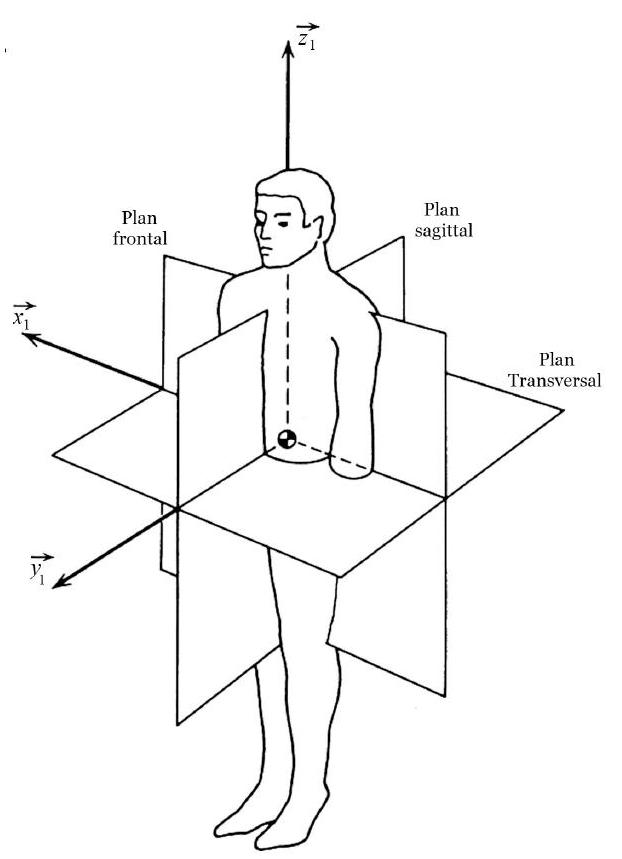
\includegraphics[max width=\textwidth]{2023_05_12_54c6a64d2ffce28d5c72g-02}
\end{center}

Figure 2 Description des plans d'évolution

\begin{center}
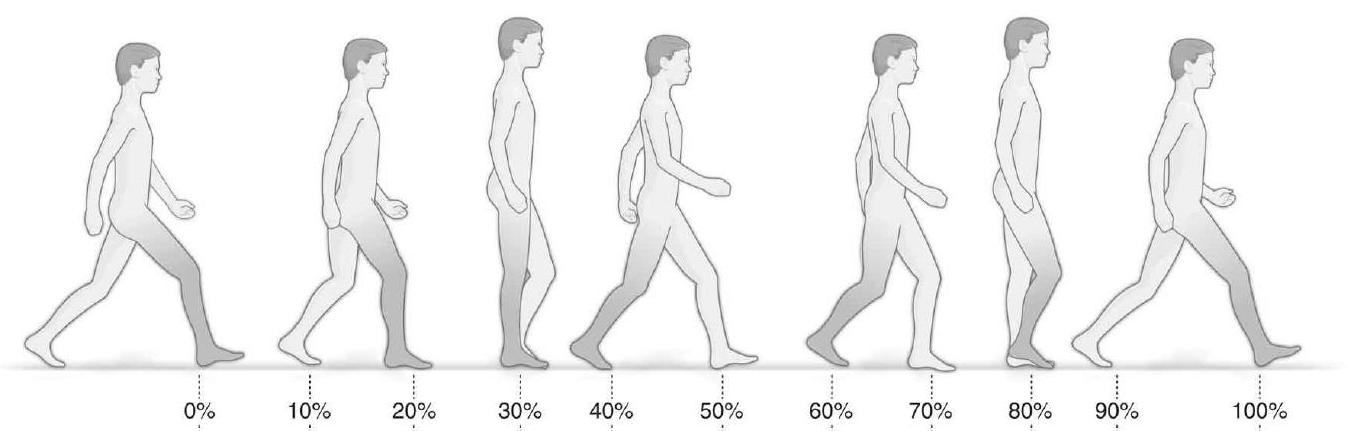
\includegraphics[max width=\textwidth]{2023_05_12_54c6a64d2ffce28d5c72g-02(1)}
\end{center}

Figure 3 Description d'une foulée en ligne droite

\section*{I Mise en évidence de la problématique lors d'une marche en ligne droite }
\begin{abstract}
Objectif Reformuler le cahier des charges global en termes de précision de façon à l'exprimer pour chacun des axes et mettre en évidence la nécessité de la prise en compte du couplage entre les axes dans la synthèse de la loi de commande.
\end{abstract}

En phase de rééducation à la proprioception de la verticalité et de la marche, il est nécessaire d'éviter la chute du patient. Des essais, menés sur des humains valides, ont permis de mettre en avant que lors d'une marche en ligne droite, une erreur de positionnement du talon de $\pm 5 \mathrm{~mm}$ risque d'amener à un déséquilibre, et donc à une chute (exigence 1.2.1.1, annexe A). Il est donc nécessaire de déterminer l'erreur de positionnement angulaire admissible sur chacun des axes de l'exosquelette pour éviter cette chute.

Dans toute l'étude, les hypothèses et notations seront les suivantes (figure 4) :

\begin{itemize}
  \item l'étude est menée dans le plan sagittal $\left(A, \vec{y}_{1}, \vec{z}_{1}\right)$, où $\vec{z}_{1}$ est vertical ascendant ;

  \item les différentes caractéristiques de dimension, masse et inertie des différents solides sont précisées annexe B ;

  \item le buste 1 étant animé d'un mouvement de translation rectiligne uniforme par rapport au référentiel terrestre, il est considéré comme galiléen ;

  \item l'étude se limite à la partie de la marche pour laquelle une des deux jambes est totalement décollée du sol (de $70 \%$ à $100 \%$ de la foulée sur la figure 3) ;

  \item le buste 1 est en liaison pivot d'axe $\left(A, \vec{x}_{1}\right)$ avec la cuisse 2 ; on note $\theta_{1}=\left(\vec{y}_{1}, \vec{y}_{2}\right)=\left(\vec{z}_{1}, \vec{z}_{2}\right)$;

  \item l'ensemble \{pied+tibia 3 , considéré comme solidaire, est en liaison pivot d'axe $\left(B, \vec{x}_{1}\right)$ avec la cuisse 2 ; on note $\theta_{2}=\left(\vec{y}_{2}, \vec{y}_{3}\right)=\left(\vec{z}_{2}, \vec{z}_{3}\right)$;

  \item les liaisons décrites précédemment sont supposées parfaites.
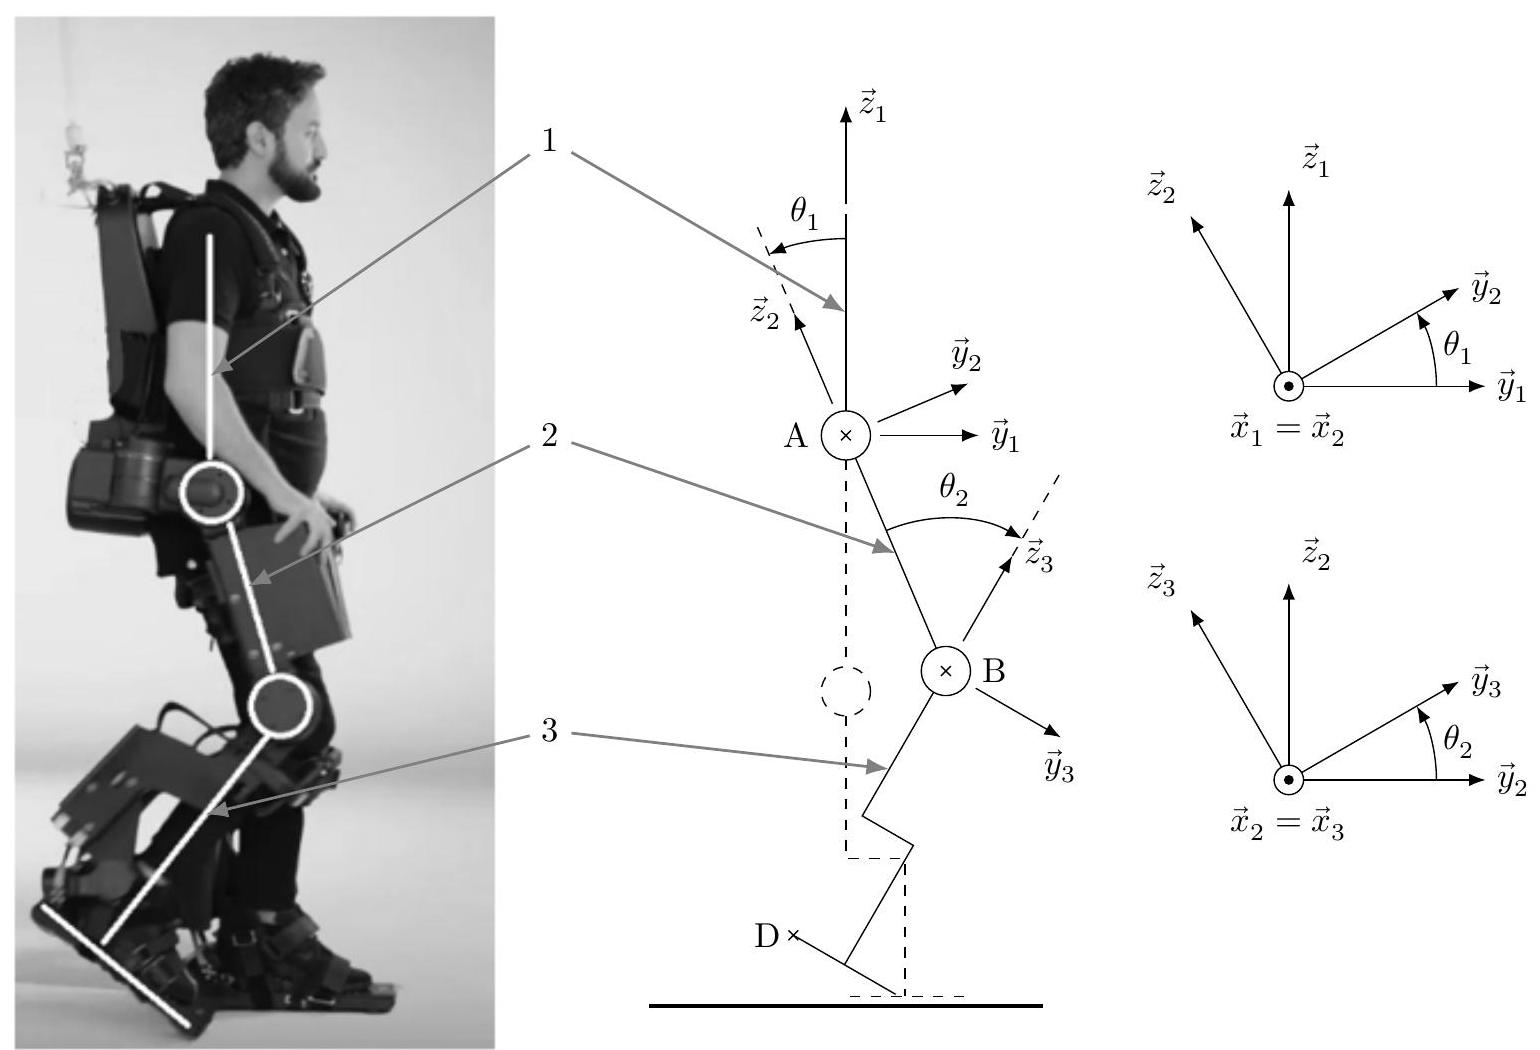
\includegraphics[max width=\textwidth, center]{2023_05_12_54c6a64d2ffce28d5c72g-03}

\end{itemize}

Figure 4 Modélisation utilisée pour la marche en ligne droite

Les positions des différents axes sont asservies à une consigne de référence afin d'obtenir la position désirée pour le point $D$ caractérisant la pointe du talon. Le cahier des charges impose que la position dans l'espace du point $D$ par rapport au point $A$ doive être celle désirée, avec une incertitude maximale de $S_{D}=5 \mathrm{~mm}$. On pose :

$$
\overrightarrow{A D}=Y \vec{y}_{1}+Z \vec{z}_{1}
$$

Q 1. Déterminer les expressions de $Y$ et $Z$, en fonction de $\theta_{1}, \theta_{2}, L_{2}$ et $L_{3}$.

L'erreur de positionnement du talon est modélisée par une variation autour d'une position connue. Cette position est paramétrée par les coordonnées $Y_{0}$ et $Z_{0}$ pour le point $D$, et par des angles $\theta_{1,0}$ et $\theta_{2,0}$ pour les liaisons pivots. Ce paramétrage se traduit, pour une variation angulaire $\Delta_{\theta}$, considérée égale sur chacun des axes, à des variations de position, $\Delta_{Y}$ et $\Delta_{Z}$, du point $D$. On suppose $\Delta_{\theta}$ faible, proche de 0 .

Q 2. À l'aide du résultat de la question 1, écrit à la position $\left(Y_{0}, Z_{0}\right)$, puis à la position $\left(Y_{0}+\Delta_{Y}, Z_{0}+\Delta_{Z}\right)$, déterminer les expressions de $\Delta_{Y}$ et $\Delta_{Z}$, en fonction de $\theta_{1,0}, \theta_{2,0}, \Delta_{\theta}, L_{2}$ et $L_{3}$.

Q 3. Déterminer alors $\Delta_{Y Z}$, la norme de la variation de positionnement total du point $D$ dans le plan $\left(\vec{y}_{1}, \vec{z}_{1}\right)$, en fonction de $\theta_{2,0}, \Delta_{\theta}, L_{2}$ et $L_{3}$.

Le résultat de la question précédente permet alors de relier l'erreur de position du talon $S_{D}$ à l'erreur de position sur les axes $S_{\theta}$, en considérant $\Delta_{Y Z}=S_{D}$ et $\Delta_{\theta}=S_{\theta}$. La figure 5 donne les évolutions sur un pas de marche de $S_{D}$ pour plusieurs valeurs de $S_{\theta}$.

Q 4. À partir de la figure 5, déterminer, parmi les valeurs proposées, l'erreur maximale admissible sur les axes $S_{\theta, \max }$ de l'exosquelette Atalante afin d'éviter la chute du patient.

Quel que soit le résultat trouvé à la question précédente, une erreur maximale admissible de 0,01 rad pour chacun des axes sera considérée pour la suite.

Afin de respecter l'exigence sur l'erreur maximale admissible, des asservissements de position et de vitesse ont été élaborés pour chacun des axes sans prendre en compte l'éventuelle influence du couplage entre les axes.

Des essais ont alors été effectués afin de mesurer l'évolution réelle des angles de chaque axe par rapport à la trajectoire visée. La figure 6 montre l'évolution de l'erreur pour l'axe de hanche sagittal de la jambe gauche lors d'une marche en ligne droite.

Q 5. À partir de la figure 6 et en justifiant la réponse, conclure sur la capacité des asservissements réalisés sans prise en compte du couplage entre les axes à respecter l'exigence 1.2.1.1.
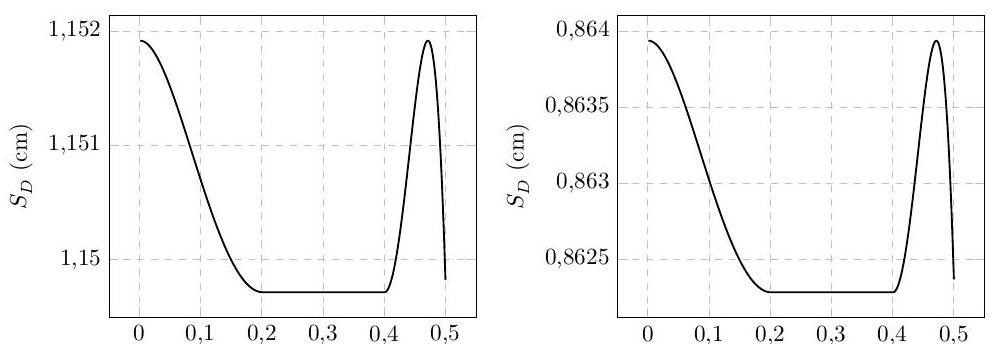
\includegraphics[max width=\textwidth, center]{2023_05_12_54c6a64d2ffce28d5c72g-04(2)}

temps (s)

\begin{center}
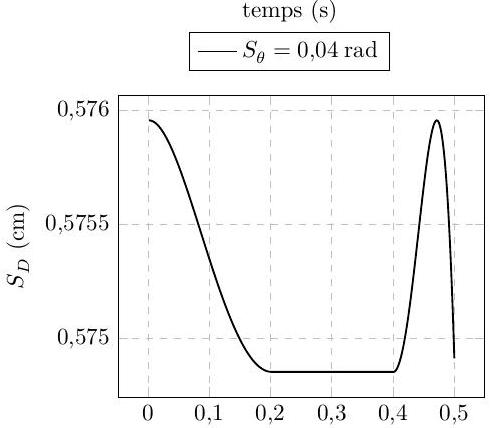
\includegraphics[max width=\textwidth]{2023_05_12_54c6a64d2ffce28d5c72g-04}
\end{center}

temps (s)

\begin{center}
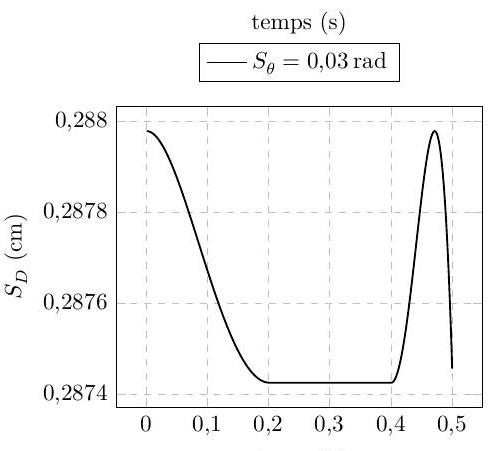
\includegraphics[max width=\textwidth]{2023_05_12_54c6a64d2ffce28d5c72g-04(4)}
\end{center}

temps (s)
$-S_{\theta}=0,02 \mathrm{rad}$

\begin{center}
\begin{tabular}{c}
temps (s) \\
$-S_{\theta}=0,01 \mathrm{rad}$ \\
\hline
\end{tabular}
\end{center}

Figure 5 Évolution de $S_{D}$ sur un pas de marche

\begin{center}
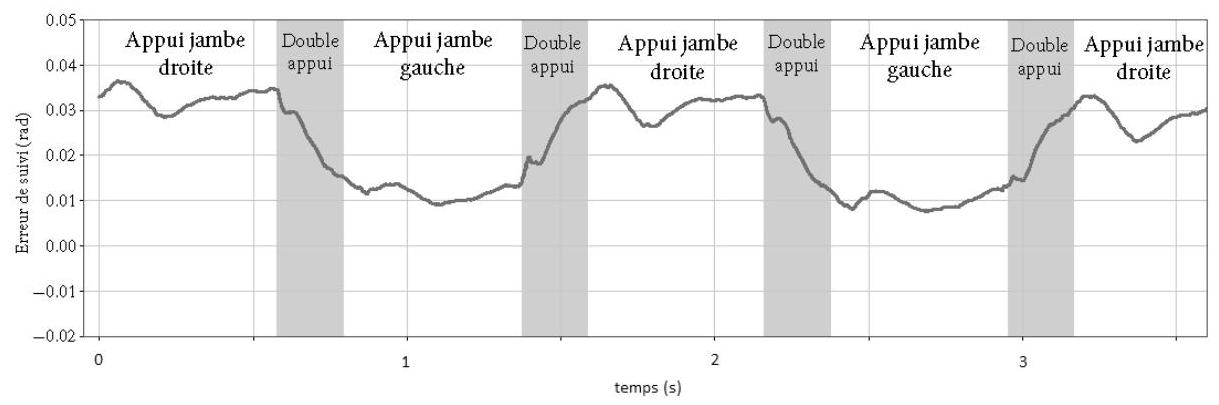
\includegraphics[max width=\textwidth]{2023_05_12_54c6a64d2ffce28d5c72g-04(3)}
\end{center}

Figure 6 Évolution de l'erreur pour l'axe de hanche sagittal de la jambe gauche

La question précédente met en avant la nécessité d'adopter une démarche de commande globale qui tient compte du couplage entre les axes. Le cahier des charges partiel de l'exosquelette concerné par cette étude (annexe A) fait apparaitre les deux exercices envisagés dans l'utilisation de l'exosquelette (renforcement musculaire et rééducation à la proprioception de la verticalité et de la marche).

Pour cela la structure envisagée de la commande s'appuie sur la figure 7 et peut être décomposée en :

\begin{itemize}
  \item un directeur de commande haut niveau (non étudié dans ce sujet). Il permet de générer en temps réel les consignes de trajectoire, ou de situation de rééducation à l'arrêt, pour chacun des axes. On suppose que ce directeur de commande, implémenté sur le buste de l'exosquelette, détermine les différentes consignes de trajectoire de manière parfaite ;

  \item une boucle interne (non linéaire). Elle a pour but de générer les actions mécaniques sur chacun des axes en fonction de la configuration d'évolution de l'exosquelette.

\end{itemize}

\begin{center}
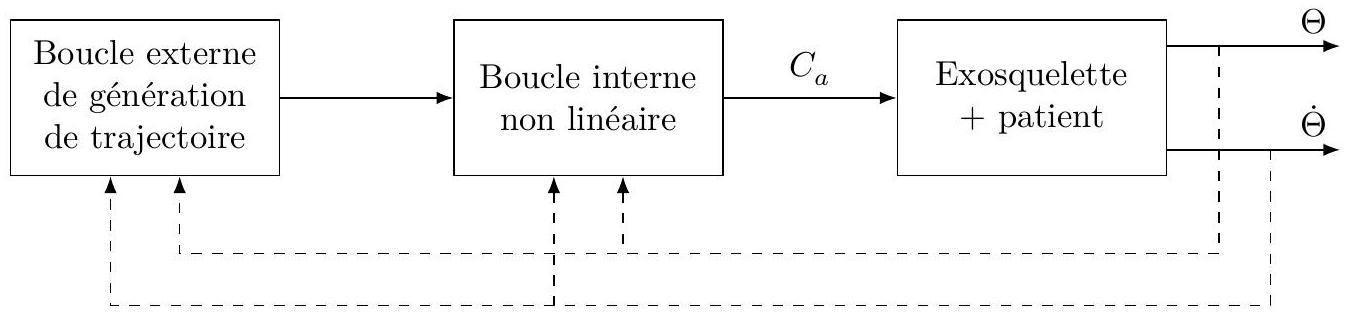
\includegraphics[max width=\textwidth]{2023_05_12_54c6a64d2ffce28d5c72g-04(1)}
\end{center}

Figure 7 Structure de commande choisie

Sur cette figure, $\Theta$ représente l'ensemble des positions angulaires des différents axes de l'exosquelette, et $C_{a}$ l'ensemble des actions mécaniques appliquées sur les différents axes.

La conception de cette commande nécessite de disposer d'un modèle dynamique de l'exosquelette. La définition et l'analyse de ce modèle dynamique seront réalisées dans la partie II. Il sera ensuite exploité dans la partie III pour la conception des lois de commande. La loi de commande dans le cas d'exercices de renforcement musculaire sera entièrement déterminée et celle dans le cas d'exercices de rééducation à la proprioception de la verticalité et de la marche sera analysée.


\end{document}